\documentclass[12pt]{article}
\usepackage[slovene]{babel}
\usepackage[utf8]{inputenc}
% \usepackage[T2A]{fontenc}
\usepackage{amsmath}
\usepackage{amsfonts}
\usepackage{amssymb}
\usepackage[version=4]{mhchem}
% \usepackage{stmaryrd}
\usepackage{graphicx}
\usepackage[export]{adjustbox}
\graphicspath{ {./images/} }
\usepackage{physics}
\usepackage{geometry}
\geometry{left=2cm,right=2cm,top=2cm,bottom=2cm}
\usepackage{parskip} 
\usepackage{float}

\title{\textbf{Spektrometrija žarkov $\gamma$ s scintilatorskim spektrometrom}}
\author{Samo Krejan}
\date{januar 2026}

\begin{document}
\maketitle

\section{Uvod}

Energije žarkov ne moremo meriti neposredno, ampak le tako da izmerimo energijo elektronov, ki jo ti prejmejo od žarkov $\gamma$ pri fotoefektu ali Comptonovem sipanju ali pa energijo tvorbo parov pozitron-elektron iz procesa tvorbe parov. Pri scintilacijskem detektorju uporabljamo v ta namen monokristale $N aJ$ z dodatkom okoli 1\% talija kot nečistoče. Pri potovanju hitrih nabitih delcev skozi kristal ostane za njimi razdejanje v obliki sledi elektron-vrzel. Ponovno združevanje med elektroni in vrzelmi poteka energijsko ugodneje v bližini atoma nečistole. Tu vrzeli vzamejo elektron atomom nečistoče in jo ionizirajo. Odvečno energijo oddajo bodisi sosednjim atomom v kristalni mreži in tako povečajo termično gibanje ali pa z izsevanje fotonov vidne svetlobe. Število scintilacijskih fotonov določimo s pomočjo fotopomnoževalke. Višina signala iz fotopomnoževalke je sorazmerna številu fotonov in torej tudi energiji, ki jo hitri nabiti delec izgubi v scintilatorju.

\subsection{Fotoefekt}

Pri fotoefektu žarek $\gamma$ izbije elektron iz enega od vezanih stanj. Najverjetneje je to elektron iz lupine K. Atom, ki je po emisiji elektrona K v vzbujenem stanju, se vrne v osnovno stanje tako, da zapolni vrzel z elektronom iz višjih stanj in pri tem izseva karakterističen žarek X. Tudi ta v scintilatorju lahko doživi fotoefekt in dobimo dva elektrona katerih energija je približno enaka prvotnemu fotou $\gamma$. Nekateri karakteristični žarki pa uidejo iz scintilatorja in s tem dobimo vrh pobega fotona pri $E = E_\gamma - E_K$ , kjer je $E_K$ vezavna energija elektrona.

\subsection{Comptonovo sipanje}

Comptonovo sipanje je neelastično sipanje fotona na skoraj prostem elektronu. Pri sipanju se seveda ohranjata energija in gibalna količina. Spekter comptonsko sipanih elektronov je zvezen.

\subsection{Tvorba parov}

Kadar ima žarek $\gamma$ dovolj energije ($E_\gamma \geq 1.02\ MeV$), se lahko v bližini jedra spremeni v par pozitron-elektron s skupno kinetično energijo $E_\gamma - 2m_0c^2$, odvečno gibalno količino pa prevzame jedro. Nastala delca se gibljeta pretežno v smeri naprej. V scintilatorju se zaustavita in mu predata svojo kinetično energijo. Ob upočasnitvi se poziton anihilira z enim od elektronov, ki jih sreča na svoji poti. Nastaneta dva kolinearna žarka $\gamma$. Možno je da pobegneta oba, samo en ali pa da oba ostaneta v scintilatorju. Tako dobimo vrh dvojnega pobega, vrh pobega in vrh polne absorbcije


\section{Potrebščine}

\begin{itemize}
    \item Scintilatorski detektor,
    \item izvor visoke napetosti za napajanje fotopomnoževalke,
    \item ojačevalnik z enokanalnim analizatorjem $Ortec 590A$,
    \item večkanalni analizator $MCA\ 8000A$,
    \item radioaktivni izvori $^{22}Na$, $^{137}Cs$ in $^{60}Co$
\end{itemize}

\section{Naloga}

\begin{itemize}
    \item S pomočjo dveh črt $\gamma$ iz $^{22}Na$ z energijo $E1 = 0.51\ MeV$ in $E2 = 1.277\ MeV$ umeri energijsko skalo scintilacijskega spektrometra in izmeri energijo črt iz $^{137}Cs$ in $^{60}Co$. Pri analizi odštej spekter ozadja
    \item Izmeri energijsko ločljivost za vrh polne absorbcije tako, da podatkom v okolici prilagajaš gaussovo funkcijo.
    \item Izračunaj izkoristek kristala za vrh polne absorbcije (določi z izvorom $^{137}Cs$)
    \item Oceni energijo vrha povratnega sipanja
\end{itemize}

\begin{figure}[H]
    \centering
    \includegraphics[width=9cm]{shema.png}
    \caption{Shema našega eksperimenta. Pod scintilatorjem postavimo radioaktivni izvor.}
\end{figure}

\section{Meritve}

Najprej sem si z osciloskopom ogledal ojačane signale iz scintilatorskega detektorja. Videl sem sliko \ref{osci}

\begin{figure}[H]
    \centering
    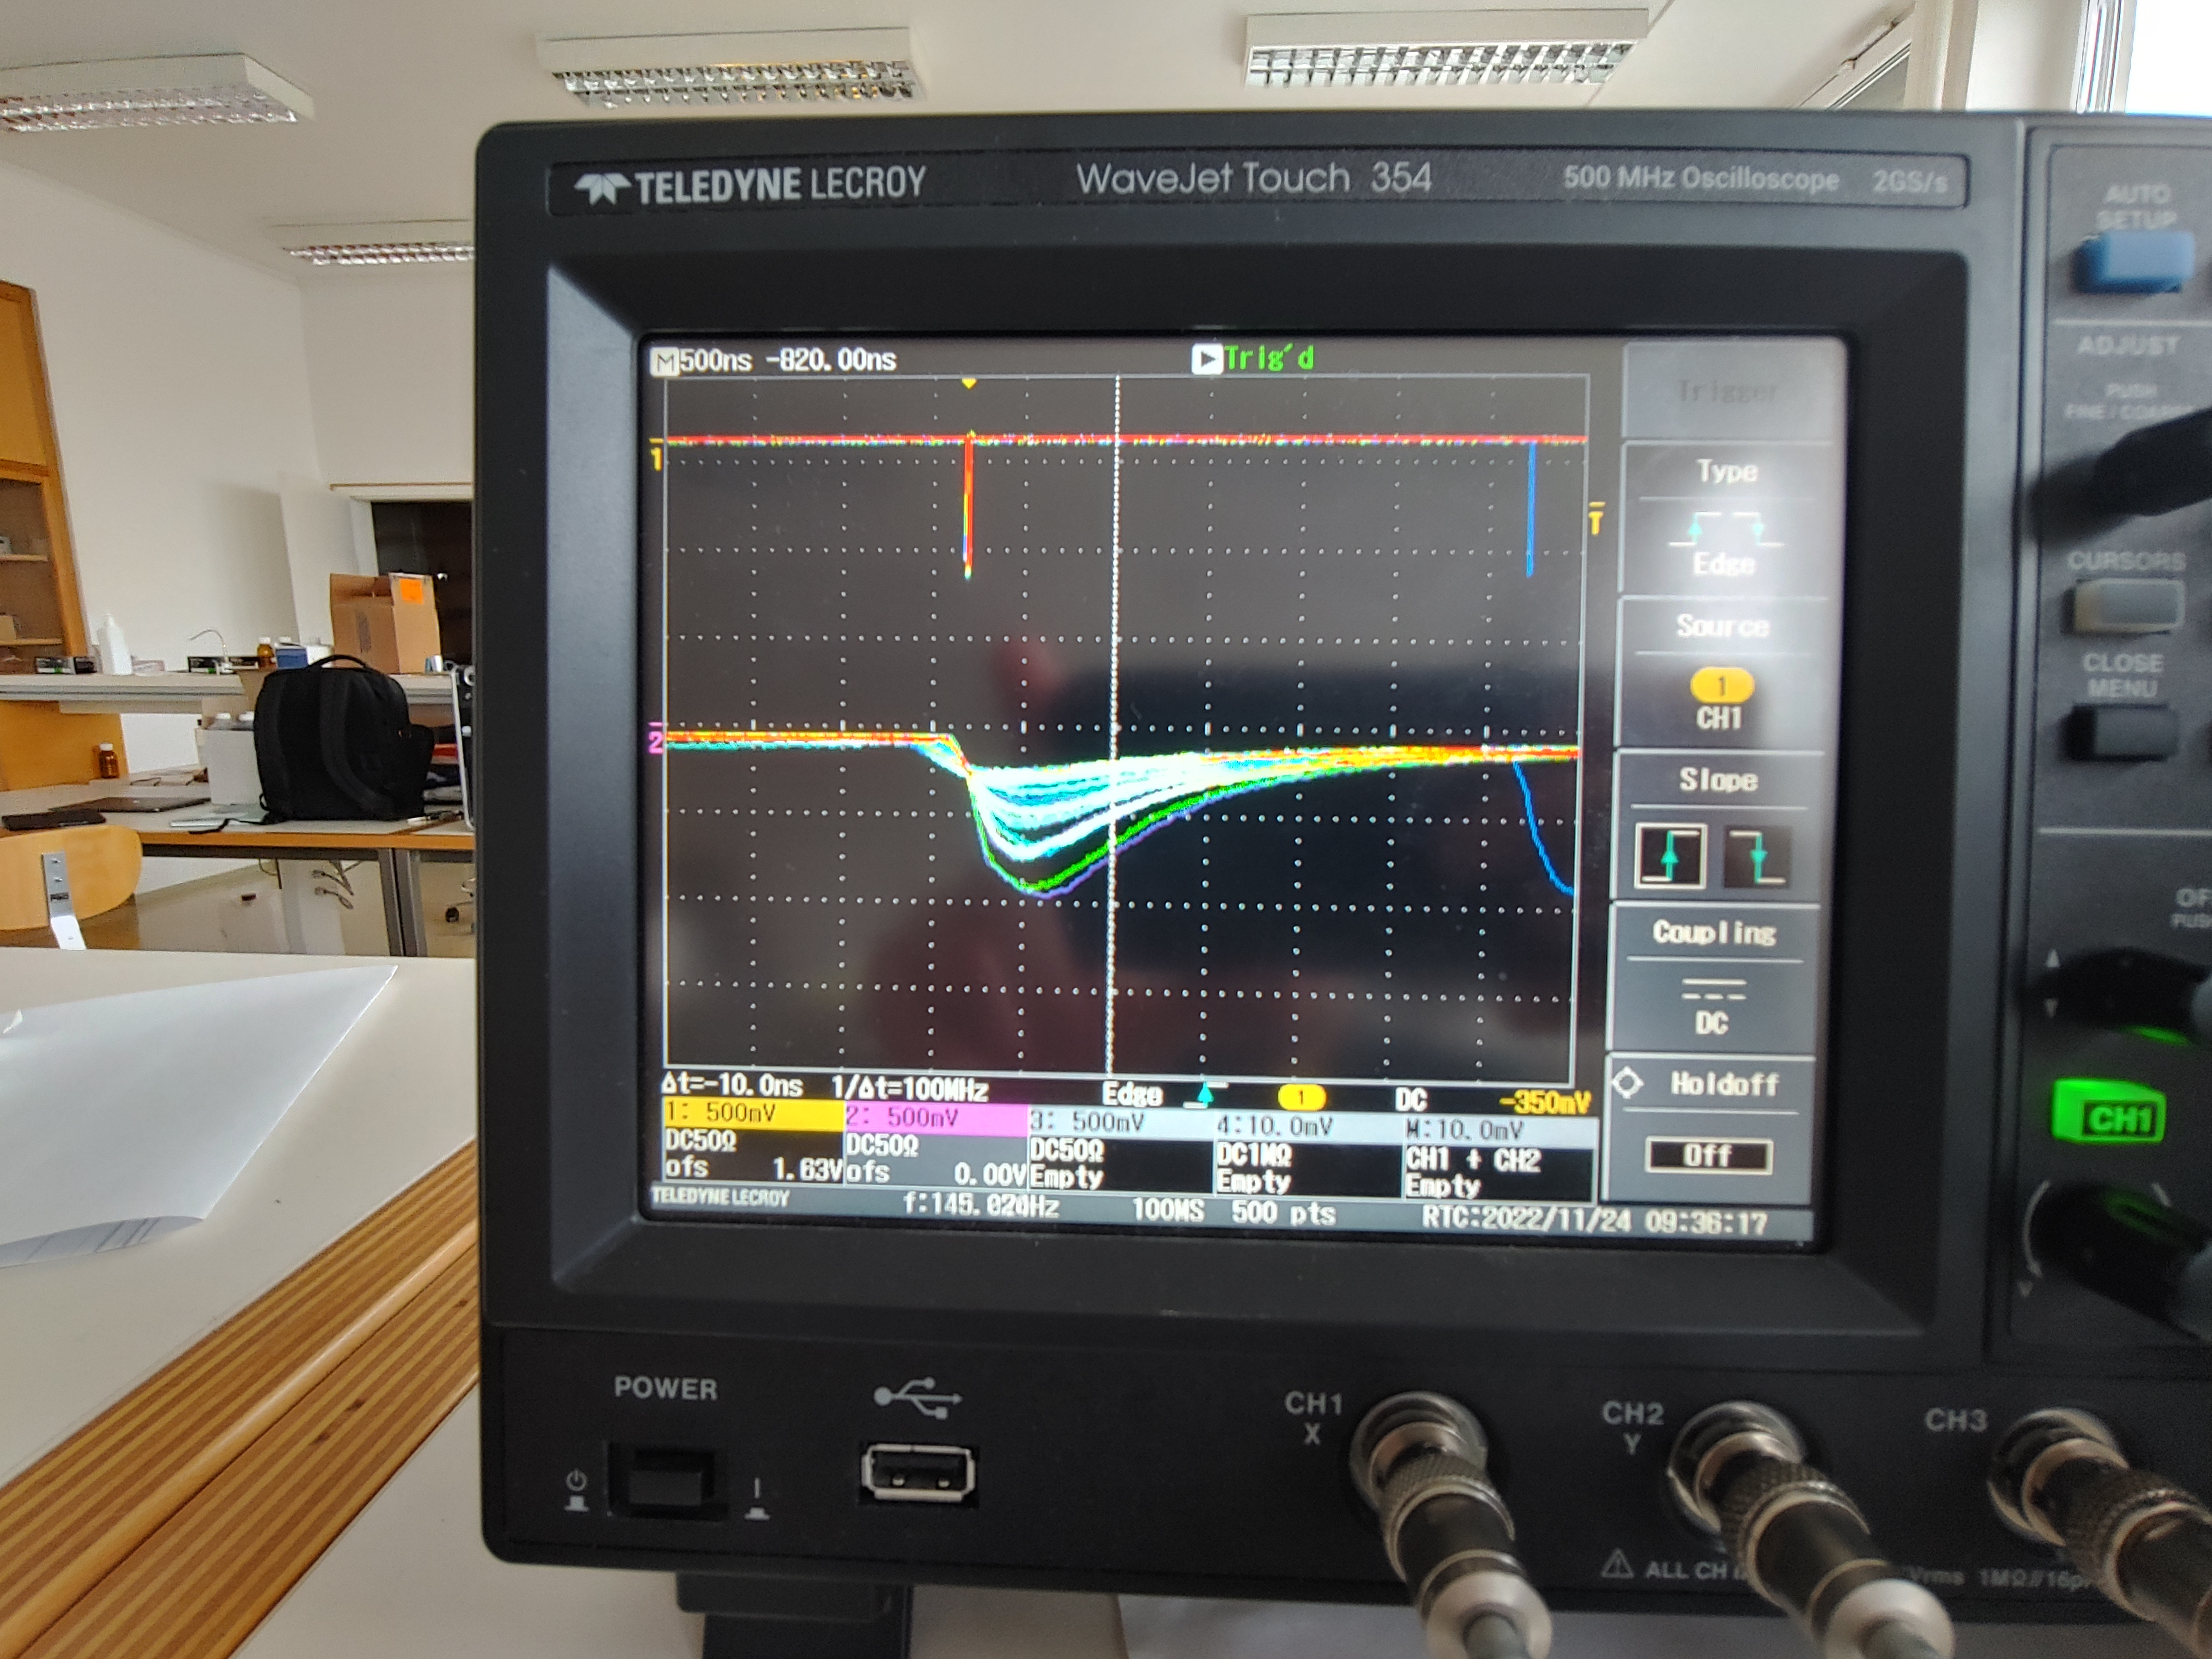
\includegraphics[width=9cm]{signal.jpg}
    \caption{Signali, sunki iz scintilatorskega detektorja na osciloskopu. Amplituda sunka je sorazmerna z energijo elektrona.}
    \label{osci}
\end{figure}

Amplituda sunka je sorazmerna z energijo elektrona. Jasno vidimo, da je ena izmed energij mnogo bolj zastopana kot ostale. V nadaljnjih meritvah to klasificiramo kot spekter.

Spekter nato pomerimo še z večkanalnim analizatorjem, ki sledi vsem energijskim (napetostnim) intervalom hkrati (slike~\ref{fig:na22},~\ref{fig:spectra}). Pomerimo tudi spekter ozadja, ki ga kasneje odštejemo od izmerjenih spektrov. Za lažje primerjanje gledamo gostoto aktivnosti, izračunamo jo tako, da število sunkov delimo s časom (\textit{livetime}) in z dolžino energijskega intervala. Na posamezne fotovrhove prilagodimo Gaussovke oblike

\begin{equation*}
    f(x) = \frac{A_0}{\sigma\sqrt{2\pi}} e^{-\frac{1}{2} \frac{x - \mu}{\sigma^2}},
\end{equation*}

katerega površina predstavlja zaznano aktivnost tega fotovrha. Vse tako izračunane aktivnosti so predstavljene na slikah~\ref{fig:na22},~\ref{fig:spectra}. Za vzorec $^{137}\mathrm{Cs}$ poznamo začetno aktivnost $9250\,\mathrm{Bq}$, izmerjeno $9 \pm 0.25$ mesecev nazaj. Če primerjamo polovico\footnote{Pokrijemo prostorski kot $2\pi$.} te aktivnosti s površino fotovrha v~\ref{fig:spectra}, izračunamo, da je učinkovitost našega detektorja

\begin{equation*}
\eta = (5.2 \pm 0.1)\,\%.
\end{equation*}

Za vse energije gamma fotonov izračunamo še predvidene položaje Comptonskega \textit{backscattering} vrha in jih prikažemo na~\ref{fig:na22},~\ref{fig:spectra}.

\begin{figure}[H]
    \begin{center}
    \includegraphics{na22-lost-spectrum.pdf}
    \end{center}
    \caption{Spekter zaznanih elektronov za $^{22}\mathrm{Na}$, izražen kot gostota aktivnosti.}
    \label{fig:na22}
\end{figure}

\begin{figure}[H]
    \begin{center}
    \includegraphics{co60-lost-spectrum.pdf}
    \includegraphics{cs137-lost-spectrum.pdf}
    \end{center}
    \caption{Spekter zaznanih elektronov za $^{60}\mathrm{Co}$ in $^{137}\mathrm{Cs}$, izražen kot gostota aktivnosti.}
    \label{fig:spectra}
\end{figure}

Povratno sevanje ocenimo kot $161\pm 9\ keV$.

\end{document}